\documentclass[11pt,a4paper]{article}

% --- Paquetes de Idioma, Fuentes y Codificación ---
\usepackage[spanish,es-tabla]{babel}
\usepackage[utf8]{inputenc}
\usepackage[T1]{fontenc}
\usepackage{helvet}
\renewcommand{\familydefault}{\sfdefault}
\usepackage{amssymb}

% --- Geometría de Página ---
\usepackage[
    a4paper,
    left=2.0cm,
    right=2.0cm,
    top=2.8cm,
    bottom=2.2cm,
    headheight=48pt,
    footskip=1.1cm
]{geometry}

% --- Elementos Gráficos, Tablas y Maquetación ---
\usepackage{graphicx}
\usepackage{xcolor}
\usepackage{booktabs}
\usepackage{tabularx}
\usepackage{array}
\usepackage{enumitem}
\usepackage{fancyhdr}
\usepackage{titlesec}
\usepackage{microtype}
\usepackage[skins,breakable]{tcolorbox}
\usepackage{lastpage}
\usepackage{hyperref}

% --- Paleta de Colores Institucionales y Ejecutivos ---
\definecolor{UtlvteNavy}{HTML}{0A2540}       % Azul marino institucional UTLVTE
\definecolor{GymPrimary}{HTML}{0284C7}       % Azul tecnológico Gym360
\definecolor{GymSecondary}{HTML}{0D9488}     % Verde azulado deportivo
\definecolor{CardBg}{HTML}{F8FAFC}           % Fondo neutro suave (Gris 50)
\definecolor{BorderGray}{HTML}{CBD5E1}       % Gris de borde sutil (Slate 300)
\definecolor{TextDark}{HTML}{1E293B}         % Texto principal de alto contraste
\definecolor{TextMuted}{HTML}{475569}        % Texto secundario explicativo
\definecolor{AccentGreen}{HTML}{16A34A}      % Verde de éxito / completado

% --- Configuración de Hipervínculos ---
\hypersetup{
    colorlinks=true,
    linkcolor=GymPrimary,
    citecolor=GymPrimary,
    urlcolor=GymPrimary,
    pdfauthor={Carrera de Tecnologías de la Información - UTLVTE - Mentor: Ing. Stalin Francis},
    pdftitle={Propuesta Ejecutiva Gym360 - Gimnasio Universitario UTLVTE}
}

% --- Configuración de Encabezados y Pies de Página ---
\pagestyle{fancy}
\fancyhf{}
\renewcommand{\headrulewidth}{0.8pt}
\renewcommand{\headrule}{\hbox to\headwidth{\color{GymPrimary}\leaders\hrule height \headrulewidth\hfill}}
\renewcommand{\footrulewidth}{0.5pt}
\renewcommand{\footrule}{\hbox to\headwidth{\color{BorderGray}\leaders\hrule height \footrulewidth\hfill}}

\fancyhead[L]{%
    \small \textbf{\color{UtlvteNavy}{UNIVERSIDAD TÉCNICA ``LUIS VARGAS TORRES'' DE ESMERALDAS}} \\
    \footnotesize \color{TextMuted}{\textbf{Facultad de Ingenierías} $\cdot$ Tecnologías de la Información $\cdot$ Mentor: Ing. Stalin Francis}%
}
\fancyhead[R]{%
    
\includegraphics[height=1.2cm]{img/logo_utlvte.png}%
}

\fancyfoot[L]{%
    \footnotesize \color{TextMuted}{\textbf{Gym360} $\cdot$ Modernización del Gimnasio Universitario $\cdot$ Mentoría: Ing. Stalin Francis}%
}
\fancyfoot[R]{%
    \footnotesize \textbf{\color{UtlvteNavy}{Página \thepage\ de \pageref{LastPage}}}%
}

% --- Estilos de Títulos y Secciones ---
\titleformat{\section}
  {\color{UtlvteNavy}\Large\bfseries}
  {\thesection.}{0.4em}{}
  [\vspace{0.8mm}{\color{GymPrimary}\hrule height 0.8pt}\vspace{1.2mm}]

\titleformat{\subsection}
  {\color{UtlvteNavy}\large\bfseries}
  {\thesubsection.}{0.3em}{}

\titlespacing*{\section}{0pt}{1.5ex plus 0.3ex minus 0.2ex}{1.0ex plus 0.2ex}
\titlespacing*{\subsection}{0pt}{1.2ex plus 0.2ex minus 0.2ex}{0.6ex plus 0.2ex}

\setlist[itemize]{leftmargin=1.3em, itemsep=0.12em, topsep=0.12em, parsep=0.06em}
\setlist[enumerate]{leftmargin=1.3em, itemsep=0.15em, topsep=0.15em, parsep=0.06em}

% --- Cajas Estilizadas para Contenido Ejecutivo ---
\tcbset{
    boxrule=0.8pt,
    arc=2.2mm,
    fonttitle=\bfseries\color{white},
    colback=white,
    boxsep=1.0mm
}

\newtcolorbox{calloutbox}[1]{
    colback=CardBg,
    colframe=GymPrimary,
    arc=2.0mm,
    boxrule=0.8pt,
    title={#1},
    coltitle=white,
    colbacktitle=GymPrimary,
    fonttitle=\bfseries\small,
    left=2.5mm,right=2.5mm,top=1.8mm,bottom=1.8mm
}

\newtcolorbox{mentorbox}[1]{
    colback=CardBg,
    colframe=UtlvteNavy,
    arc=2.2mm,
    boxrule=1.0pt,
    title={#1},
    coltitle=white,
    colbacktitle=UtlvteNavy,
    fonttitle=\bfseries\small,
    left=3mm,right=3mm,top=2mm,bottom=2mm
}

\newtcolorbox{screenshotcard}[1]{
    colback=white,
    colframe=BorderGray,
    arc=2.0mm,
    boxrule=0.6pt,
    title={\footnotesize \textbf{\color{UtlvteNavy}{#1}}},
    coltitle=UtlvteNavy,
    colbacktitle=CardBg,
    left=1mm,right=1mm,top=1mm,bottom=1mm
}

% --- Inicio del Documento ---
\begin{document}

% =========================================================================
% PÁGINA 1: MEMORANDO EJECUTIVO Y RESUMEN GENERAL
% =========================================================================
\begin{tcolorbox}[colback=CardBg, colframe=UtlvteNavy, boxrule=1.2pt, arc=3.0mm, left=4.5mm, right=4.5mm, top=3.5mm, bottom=3.5mm]
    \begin{minipage}[c]{0.78\textwidth}
        {\Large \textbf{\color{UtlvteNavy}{PROPUESTA EJECUTIVA INSTITUCIONAL}}}\\[1.2mm]
        {\large \textbf{\color{GymPrimary}{Proyecto: Sistema de Gestión Deportiva ``Gym360''}}}\\[0.8mm]
        {\normalsize \textbf{\color{TextDark}{Modernización y Control Integral del Gimnasio Universitario UTLVTE}}}\\[0.8mm]
        {\footnotesize \color{TextMuted}{\textbf{Alianza de Cooperación:} Carrera de Cultura Física $\longleftrightarrow$ Carrera de Tecnologías de la Información}}
    \end{minipage}
    \hfill
    \begin{minipage}[c]{0.18\textwidth}
        \centering
        
\includegraphics[width=\linewidth]{img/logo_utlvte.png}
    \end{minipage}

    \vspace{2mm}
    {\color{BorderGray}\hrule height 0.6pt}
    \vspace{2mm}

    % Datos institucionales del memorando
    \renewcommand{\arraystretch}{1.18}
    \begin{tabularx}{\linewidth}{@{}p{1.8cm}X@{}}
        \textbf{\color{UtlvteNavy}{PARA:}} & \textbf{Lcda. Vilma Viviana García Caicedo} \newline 
        {\footnotesize Directora de la Carrera de Cultura Física (Pedagogía de la Actividad Física y Deporte) $\cdot$ UTLVTE} \\[1.2mm]
        \textbf{\color{UtlvteNavy}{DE:}} & \textbf{Equipo de Desarrollo de Software $\cdot$ Asignatura: Ingeniería de Software} \newline 
        \textbf{\color{UtlvteNavy}{DOCENTE GUÍA Y MENTOR:}} \textbf{\color{GymPrimary}{Ing. Stalin Francis}} \newline
        {\footnotesize Carrera de Tecnologías de la Información $\cdot$ Facultad de Ingenierías $\cdot$ UTLVTE} \\[1.2mm]
        \textbf{\color{UtlvteNavy}{ASUNTO:}} & \textbf{Propuesta de Implementación de Gym360 y Demostración Gráfica de Alto Valor (Sprint 1)} \\[1.2mm]
        \textbf{\color{UtlvteNavy}{FECHA:}} & Octubre de 2026 $\cdot$ Esmeraldas, Ecuador \\
    \end{tabularx}
\end{tcolorbox}

\vspace{2.5mm}

\section{Resumen Ejecutivo: El Propósito en Pocas Palabras}

Estimada Lcda. Vilma Viviana García Caicedo:

El gimnasio de la \textbf{Universidad Técnica ``Luis Vargas Torres'' de Esmeraldas} es un espacio central para el bienestar institucional: en él convergen nuestros deportistas de selección, docentes, servidores universitarios y, de manera muy especial, los estudiantes de la carrera de \textbf{Cultura Física}, quienes encuentran en estas instalaciones su taller de formación práctica profesional.

Con la meta de respaldar su gestión directiva y transformar la administración del gimnasio en un modelo de eficiencia, modernidad y transparencia, desde la carrera de \textbf{Tecnologías de la Información}, bajo el liderazgo académico, supervisión metodológica y mentoría experta del docente \textbf{Ing. Stalin Francis} en la cátedra de \textbf{Ingeniería de Software}, ponemos a su consideración la adopción e implementación de la plataforma:

\begin{center}
    \colorbox{CardBg}{\parbox{0.96\linewidth}{
        \centering \vspace{1.8mm}
        {\Large \textbf{\color{GymPrimary}{Gym360: Plataforma Digital para el Gimnasio Universitario}}}\\[1.2mm]
        \textit{\color{TextDark}{Un sistema moderno, ágil y visualmente intuitivo que sustituye las planillas físicas de papel por un control digitalizado del acceso y aforo en tiempo real, monitoreo patrimonial del equipamiento con fotografías reales, un atlas pedagógico de 27 grupos musculares y un catálogo interactivo de más de 1,000 ejercicios anatómicos para docentes y entrenadores.}}
        \vspace{1.8mm}
    }}
\end{center}

Esta iniciativa parte de un hecho concreto: \textbf{Gym360 no es un proyecto en papel ni una idea teórica, sino un sistema real cuyo Primer Sprint se encuentra 100\% implementado, probado y en funcionamiento pleno en servidor local}. 

A través de esta propuesta ejecutiva, estructurada con capturas reales y gráficos de alto valor analítico, le exponemos el diagnóstico institucional, las soluciones desarrolladas bajo la mentoría del \textbf{Ing. Stalin Francis} y los beneficios directos para su carrera y nuestra universidad.

\newpage

% =========================================================================
% PÁGINA 2: DIAGNÓSTICO COMPARATIVO Y ENFOQUE METODOLÓGICO
% =========================================================================
\section{Diagnóstico: De la Gestión Manual a la Excelencia Digital}

Tradicionalmente, el control de instalaciones deportivas en instituciones de educación superior se ha realizado mediante registros manuales en papel. Aunque comprensibles en su momento, hoy generan pérdida de tiempo, falta de datos estadísticos y riesgos de desorganización. 

La siguiente tabla resume de forma clara cómo \textbf{Gym360} supera estos problemas en el día a día:

\vspace{1mm}
\begin{center}
\renewcommand{\arraystretch}{1.1}
\begin{tabularx}{\linewidth}{@{}>{\raggedright\bfseries\color{UtlvteNavy}}p{2.6cm} >{\raggedright\small}X >{\raggedright\arraybackslash\small}X@{}}
\toprule
\textbf{\normalsize Área del Gimnasio} & \textbf{\normalsize \color{TextMuted}{Gestión Manual Tradicional}} & \textbf{\normalsize \color{GymSecondary}{Solución Inteligente con Gym360}} \\
\midrule
\textbf{1. Ficha del Usuario} & Fichas en papel deterioradas y extraviadas. & \textbf{Expediente digital único:} Búsqueda en 2 seg.; contactos de emergencia siempre visibles. \\
\addlinespace
\textbf{2. Asistencia y Aforo} & Cuadernos sin hora de salida ni conteo. & \textbf{Control de entrada y salida:} Registro exacto de permanencia y control de aforo en vivo. \\
\addlinespace
\textbf{3. Máquinas y Pesas} & Sin alertas ni control de vida útil. & \textbf{Inventario fotográfico activo:} 60 equipos con foto real, código y ficha de mantenimiento. \\
\addlinespace
\textbf{4. Planificación Física} & Rutinas verbales con riesgo de lesiones. & \textbf{Atlas anatómico y biomecánico:} 27 músculos y 1,058 ejercicios con fases Start/Peak y video. \\
\addlinespace
\textbf{5. Informes de Gestión} & Semanas consolidando datos manualmente. & \textbf{Reportes analíticos en 1 clic:} Gráficos interactivos para Decanato y acreditación CACES. \\
\bottomrule
\end{tabularx}
\end{center}

\vspace{1.5mm}

\section{Metodología de Desarrollo y Mentoría Académica}

En la ingeniería de software moderna, los proyectos de alto impacto se rigen bajo metodologías ágiles (\textit{Scrum}). Bajo la mentoría y guía técnica del docente \textbf{Ing. Stalin Francis}, los estudiantes aplican estándares rigurosos de arquitectura MVC, modelado relacional y experiencia de usuario (UX/UI). 

\vspace{1mm}

\begin{mentorbox}{Liderazgo y Mentoría del Docente Guía: Ing. Stalin Francis}
La concepción, modelado y control de calidad de \textbf{Gym360} han sido orientados y supervisados directamente por el docente \textbf{Ing. Stalin Francis}, quien ha inculcado al equipo una visión práctica orientada a resolver las necesidades reales de nuestra universidad. Su guía técnica asegura escalabilidad, seguridad y máxima utilidad pedagógica para Cultura Física.

\vspace{1.2mm}
{\color{BorderGray}\hrule height 0.5pt}\vspace{1.2mm}
\textbf{\color{AccentGreen}{Hito Alcanzado $\checkmark$ Primer Sprint Operativo al 100\%:}}
Bajo su dirección, el equipo culminó con éxito el núcleo del software: panel ejecutivo con analítica visual, base unificada de usuarios, control de asistencias, inventario fotográfico de 60 máquinas, atlas anatómico de 27 músculos y prescripción individual de rutinas. En las siguientes páginas se exhiben las pantallas reales del sistema.
\end{mentorbox}

\newpage

% =========================================================================
% PÁGINA 3: SPRINT 1 - DASHBOARD Y FICHA DEL DEPORTISTA
% =========================================================================
\section{Resultados Tangibles: Pantallas y Gráficos de Alto Valor}

\subsection{Panel de Control Ejecutivo (Dashboard 360): Analítica Visual en Tiempo Real}
\textbf{¿Para qué sirve?:} Es la sala de control central que permite a la Dirección de Carrera y a los administradores conocer al instante el estado del gimnasio mediante gráficos analíticos interactivos: distribución del inventario de equipamiento (cardiovascular, fuerza, peso libre, funcional) y cobertura biomecánica por grupos musculares, facilitando la toma de decisiones informadas.

\vspace{1mm}
\noindent
\begin{screenshotcard}{Figura 1: Panel de Control Ejecutivo de Gym360 con Métricas Clave y Gráficos Analíticos de Inventario y Biomecánica}
    \centering
    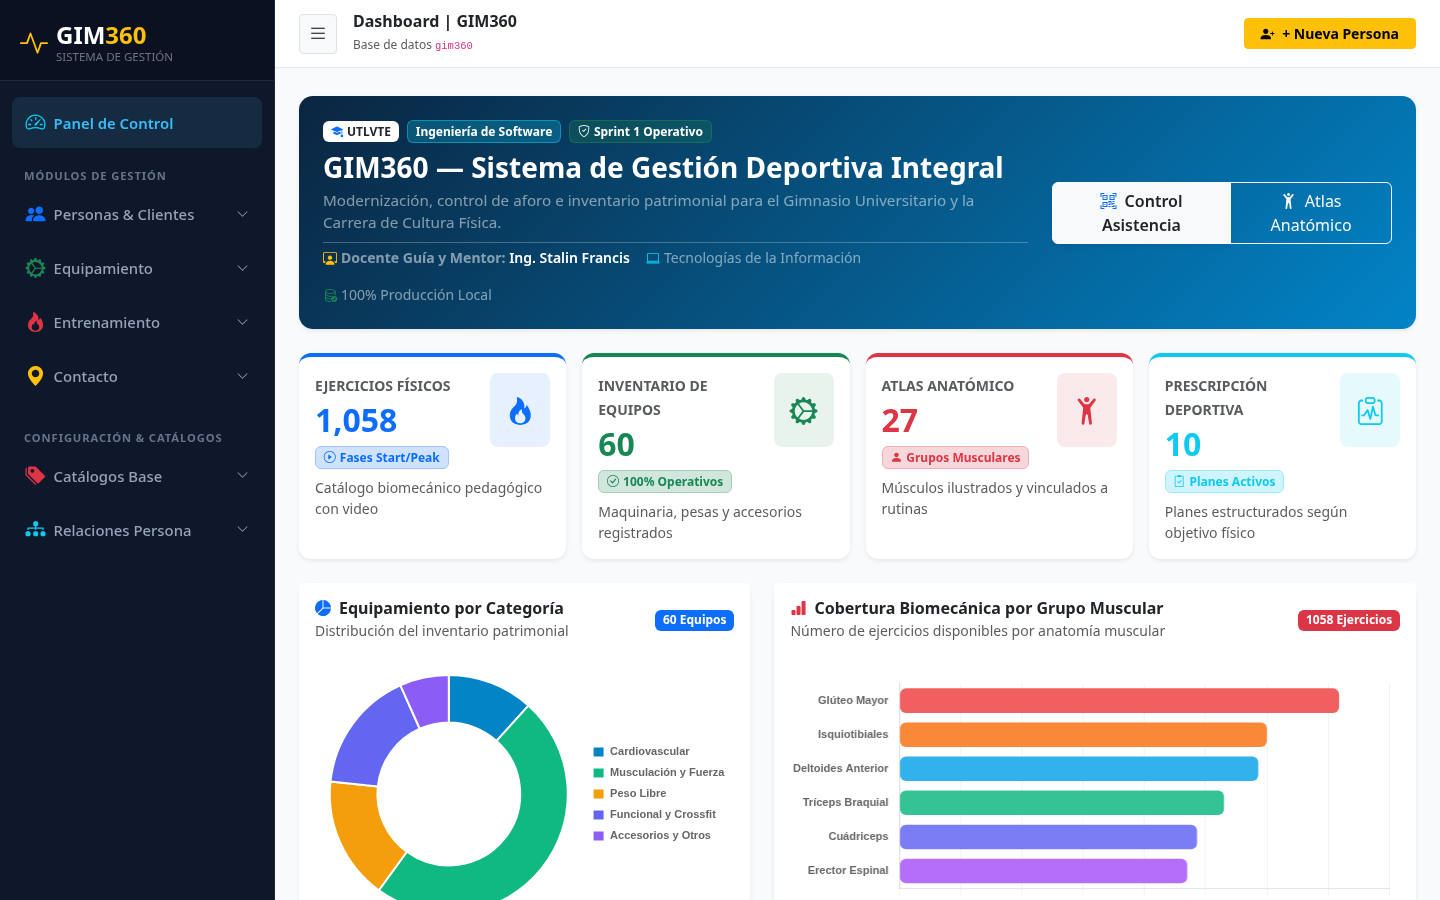
\includegraphics[width=\linewidth,height=5.8cm,keepaspectratio]{img/screenshot_dashboard.png}
\end{screenshotcard}

\vspace{2.5mm}

\subsection{Ficha Única del Deportista y Usuario Universitario (Módulo Personas)}
\textbf{¿Para qué sirve?:} Centraliza el expediente de estudiantes de Cultura Física, selecciones deportivas de la UTLVTE, docentes y personal institucional. Registra cédula, nombres, correo, dirección domiciliaria, estado civil e identidad de género, permitiendo habilitar membresías con un solo clic. Como muestra de validación real, se exhibe el registro del docente mentor \textbf{Ing. Stalin Francis}.

\vspace{1mm}
\noindent
\begin{screenshotcard}{Figura 2: Expediente Digital Único del Deportista y Usuario Institucional (Registro de Validación: Ing. Stalin Francis)}
    \centering
    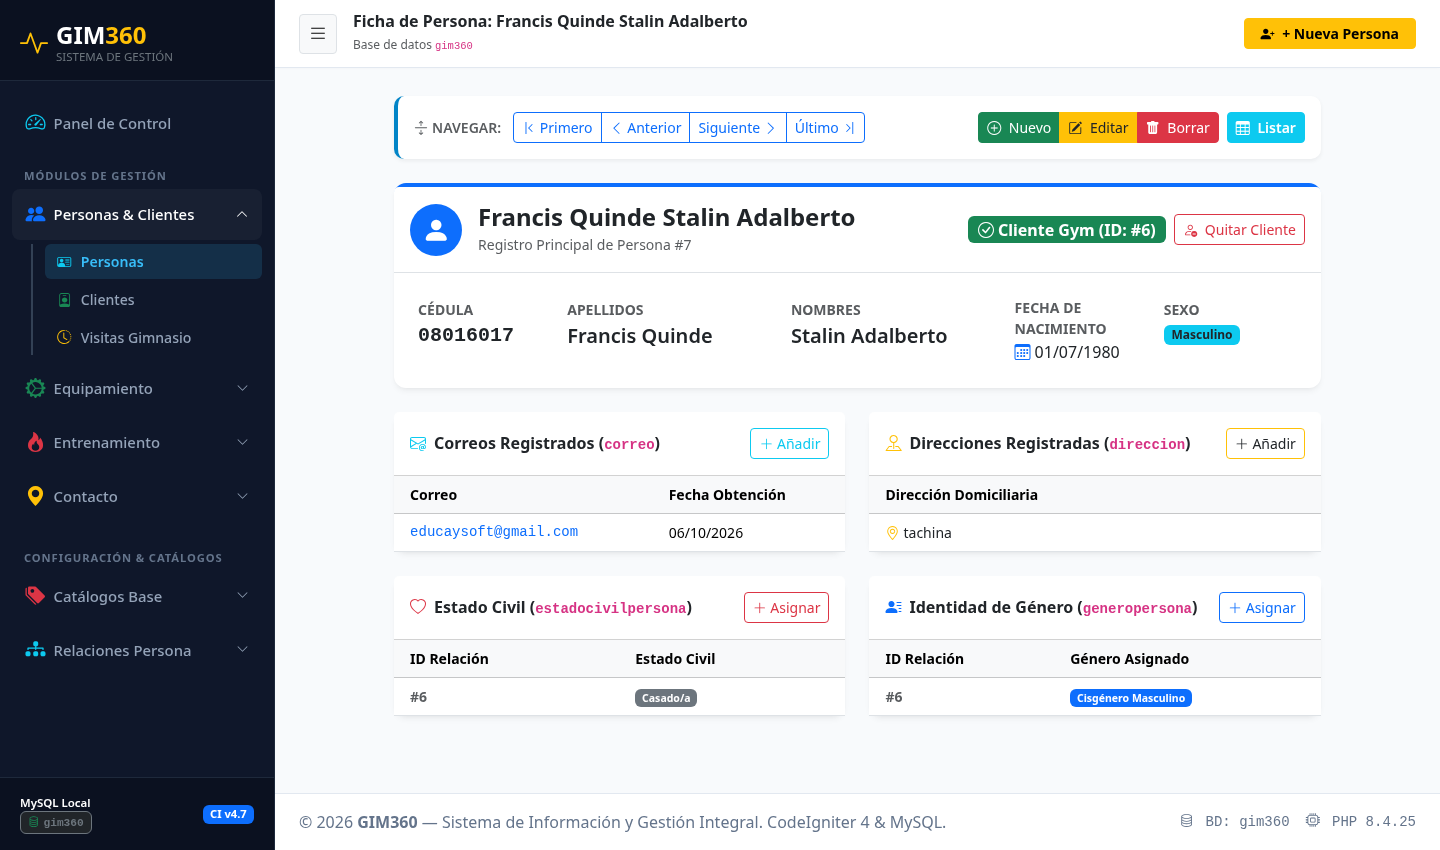
\includegraphics[width=\linewidth,height=5.8cm,keepaspectratio]{img/screenshot_personas.png}
\end{screenshotcard}

\newpage

% =========================================================================
% PÁGINA 4: SPRINT 1 - ASISTENCIAS E INVENTARIO DE EQUIPOS
% =========================================================================
\subsection{Control Inteligente de Asistencia y Aforo en Tiempo Real (Módulo Visitas)}
\textbf{¿Para qué sirve?:} Registra con exactitud cronológica la fecha, hora exacta de entrada, hora de salida y tiempo de permanencia de cada usuario. Permite supervisar el aforo seguro de las salas para evitar sobrecupos y certificar las horas prácticas que los estudiantes de Cultura Física deben cumplir durante su ciclo formativo.

\vspace{1mm}
\noindent
\begin{screenshotcard}{Figura 3: Bitácora Histórica y Control Diario de Asistencias con Horas de Ingreso, Salida y Tiempos de Estadía}
    \centering
    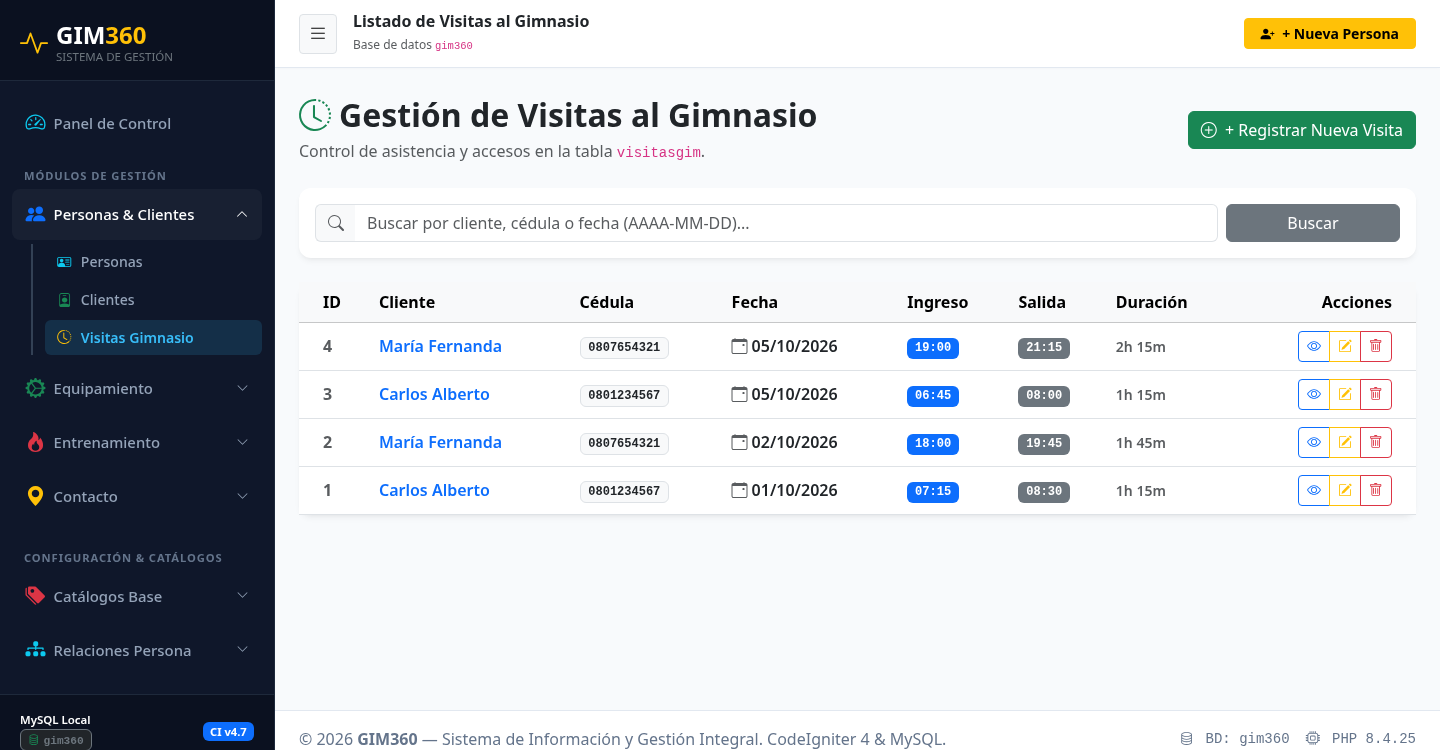
\includegraphics[width=\linewidth,height=5.8cm,keepaspectratio]{img/screenshot_visitas.png}
\end{screenshotcard}

\vspace{2.5mm}

\subsection{Inventario Fotográfico y Patrimonial de Maquinaria Deportiva (Módulo Equipos)}
\textbf{¿Para qué sirve?:} Salvaguarda el patrimonio deportivo de la universidad registrando cada máquina, aparato cardiovascular, banco o accesorio con su código interno, fotografía real, marca, modelo, ubicación física y estado operativo (100\% operativo y excelente en las 60 máquinas actuales), facilitando la programación de mantenimientos preventivos.

\vspace{1mm}
\noindent
\begin{screenshotcard}{Figura 4: Ficha Técnica Patrimonial con Fotografía Real de Maquinaria y Control de Estado Operativo}
    \centering
    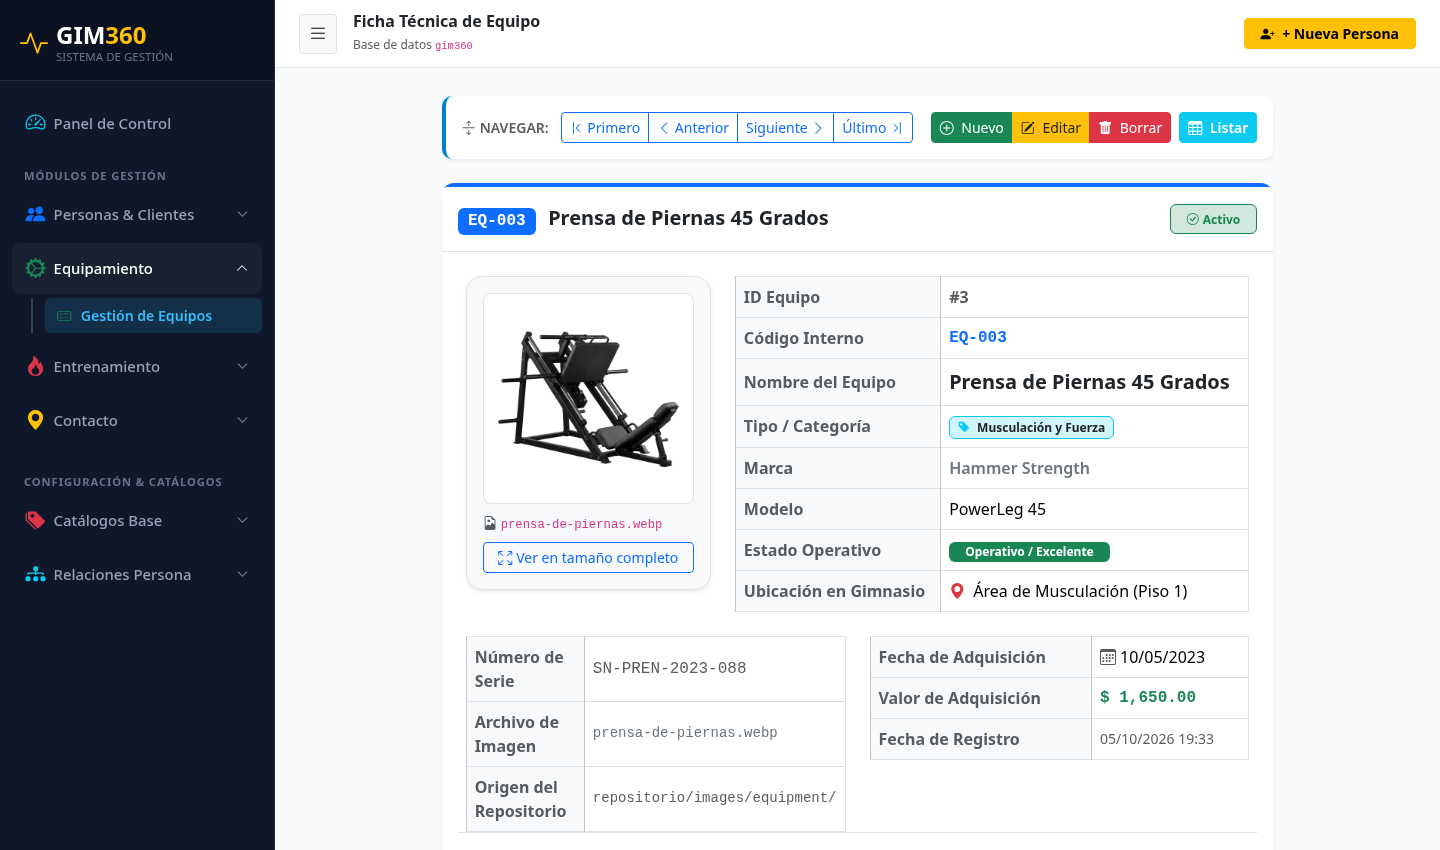
\includegraphics[width=\linewidth,height=5.8cm,keepaspectratio]{img/screenshot_equipos.png}
\end{screenshotcard}

\newpage

% =========================================================================
% PÁGINA 5: SPRINT 1 - ATLAS MUSCULAR Y CATÁLOGO DE EJERCICIOS
% =========================================================================
\subsection{Atlas Anatómico Muscular Interactivo (Módulo Músculos)}
\textbf{¿Para qué sirve?:} Constituye un soporte pedagógico de primer nivel concebido especialmente para las cátedras de Anatomía Funcional, Biomecánica y Entrenamiento Deportivo de la carrera de \textbf{Cultura Física}. Ofrece una galería visual interactiva con los 27 grupos musculares del cuerpo humano aislados y clasificados para consulta didáctica en clase.

\vspace{1mm}
\noindent
\begin{screenshotcard}{Figura 5: Atlas Anatómico Gráfico Integrado con 27 Grupos Musculares Ilustrados para Docencia Deportiva}
    \centering
    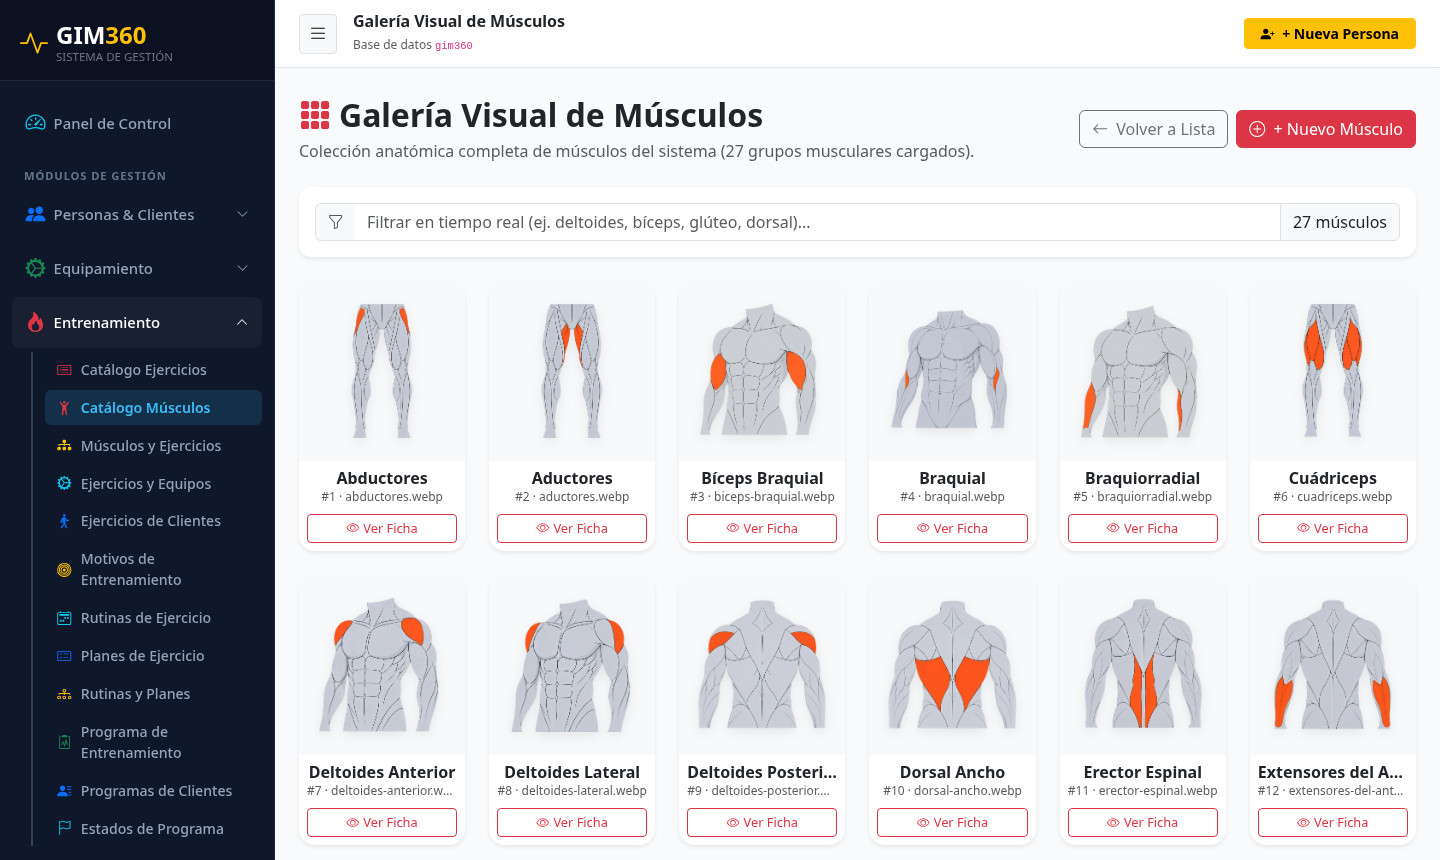
\includegraphics[width=\linewidth,height=5.8cm,keepaspectratio]{img/screenshot_musculos.png}
\end{screenshotcard}

\vspace{2.5mm}

\subsection{Catálogo Biomecánico de Ejercicios Físicos (Módulo Ejercicios)}
\textbf{¿Para qué sirve?:} Pone a disposición de entrenadores y estudiantes un catálogo de más de 1,000 ejercicios clasificados biomecánicamente. Cada ejercicio incluye ilustración de la postura inicial (\textit{Start}) y pico de contracción (\textit{Peak}), video tutorial demostrativo y la vinculación directa con los músculos activados y las máquinas requeridas para su ejecución.

\vspace{1mm}
\noindent
\begin{screenshotcard}{Figura 6: Ficha Biomecánica de Ejercicio con Fases de Movimiento, Video Demostrativo y Músculos Involucrados}
    \centering
    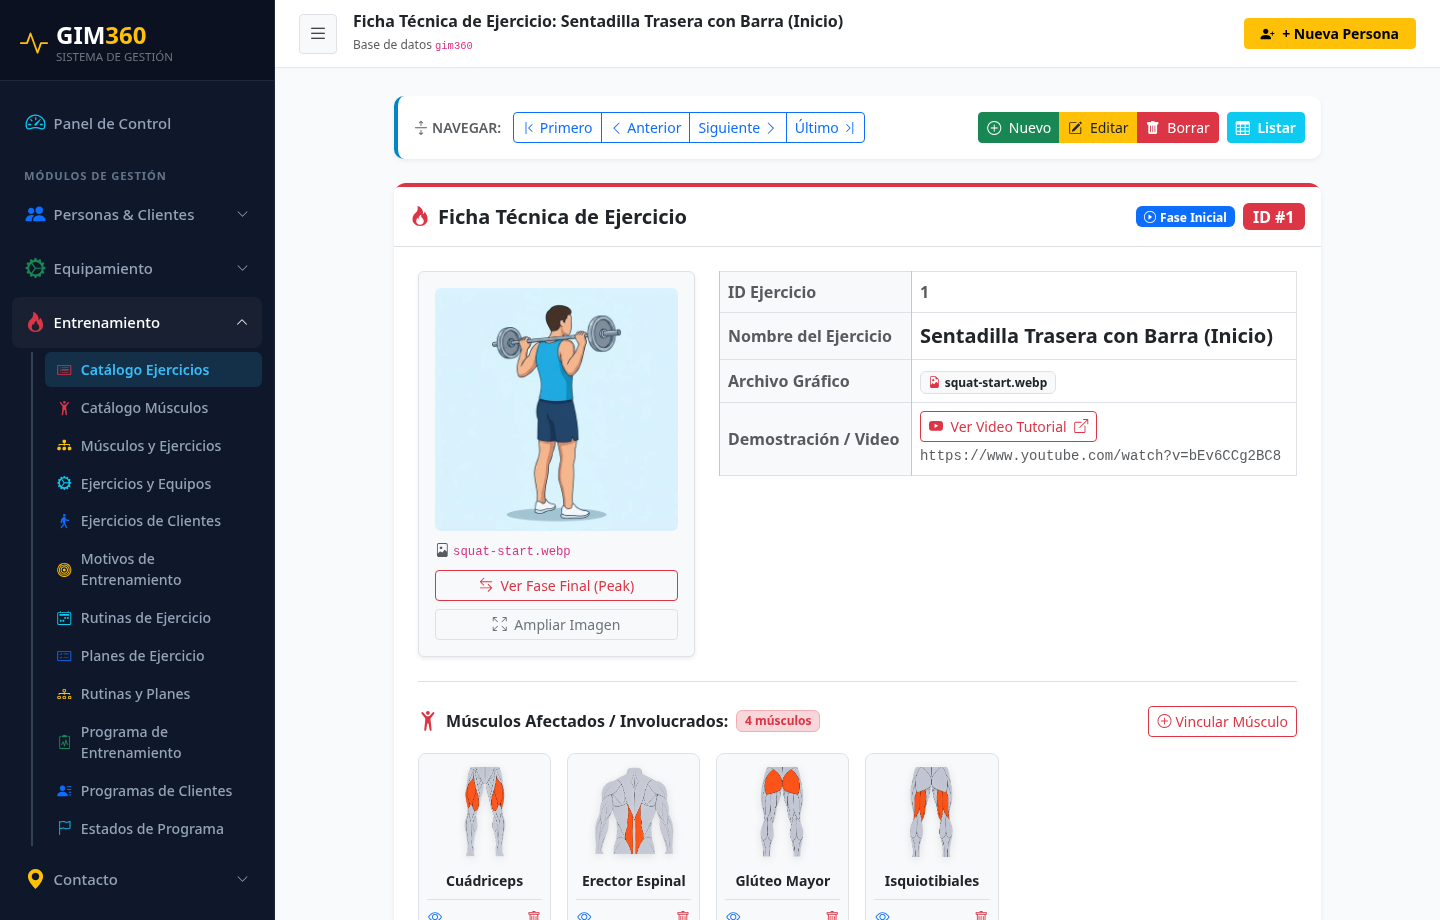
\includegraphics[width=\linewidth,height=5.8cm,keepaspectratio]{img/screenshot_ejercicios.png}
\end{screenshotcard}

\newpage

% =========================================================================
% PÁGINA 6: PRESCRIPCIÓN DEPORTIVA Y PROGRAMAS DE ENTRENAMIENTO
% =========================================================================
\subsection{Prescripción Deportiva y Programas Personalizados de Entrenamiento}
\textbf{¿Para qué sirve?:} Es una de las herramientas más valiosas para los docentes y entrenadores de la carrera de \textbf{Cultura Física}. Permite asignar planes de entrenamiento individualizados a cada deportista o estudiante según su objetivo específico (hipertrofia muscular, pérdida de grasa/definición, resistencia cardiovascular o fuerza máxima). 

El sistema detalla la rutina prescrita, los días por semana de práctica, el número de series, repeticiones recomendadas, intervalos de descanso entre series, cargas sugeridas (en kilogramos) y las indicaciones técnicas posturales para una ejecución biomecánicamente segura y efectiva.

\vspace{1.5mm}
\noindent
\begin{screenshotcard}{Figura 7: Ficha Digital de Prescripción y Asignación de Programa de Entrenamiento Personalizado al Deportista}
    \centering
    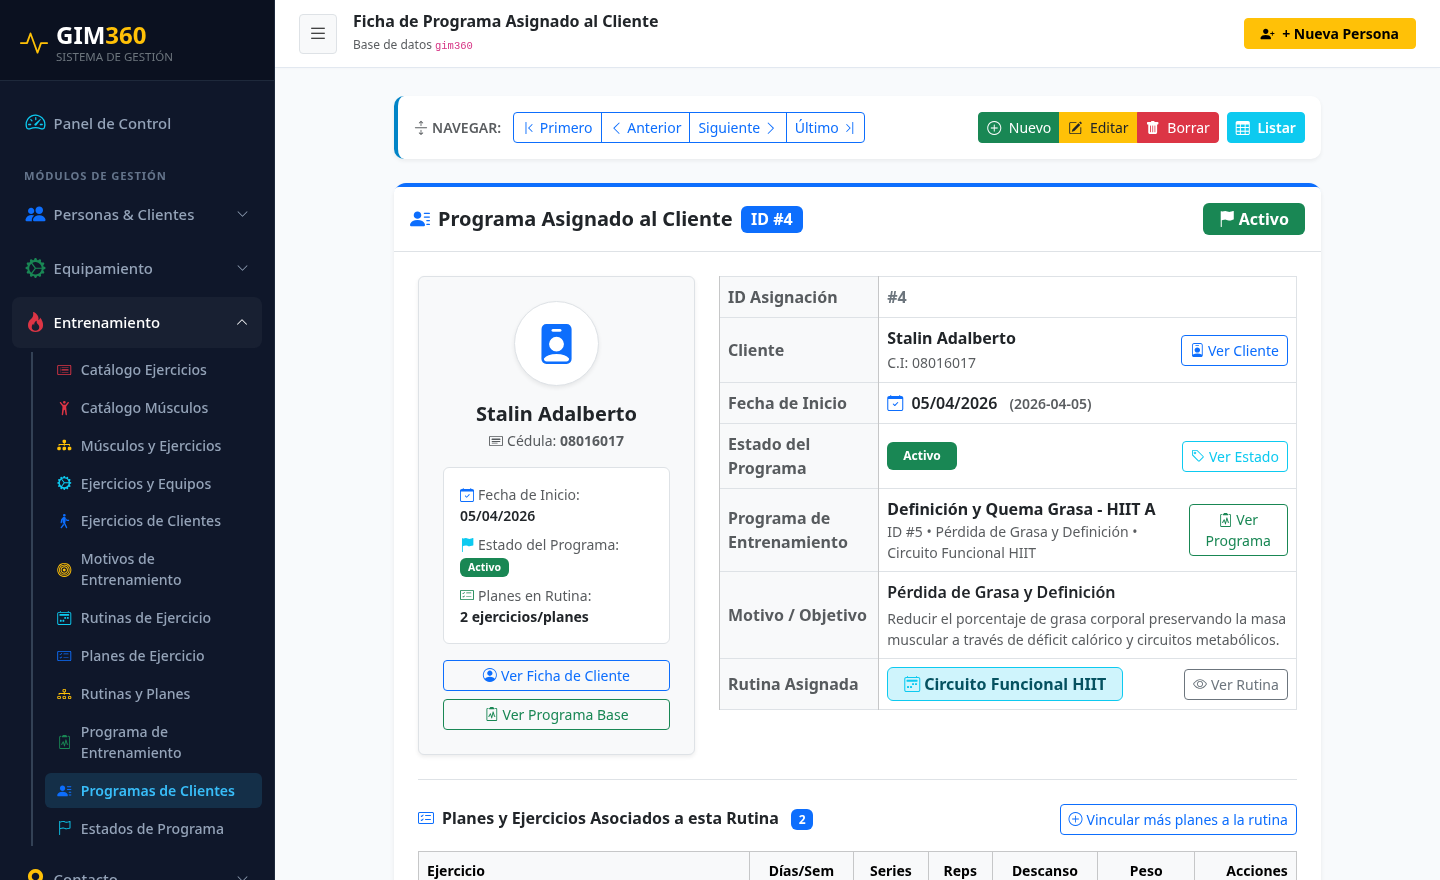
\includegraphics[width=\linewidth,height=6.2cm,keepaspectratio]{img/screenshot_programa.png}
\end{screenshotcard}

\vspace{2.5mm}

\begin{calloutbox}{Impacto Didáctico Directo para Cultura Física}
Este módulo convierte al gimnasio universitario en un verdadero laboratorio práctico: los estudiantes de Cultura Física aprenden a formular prescripciones de ejercicio bajo parámetros científicos validados y pueden realizar el seguimiento en vivo del progreso de sus compañeros y atletas de selección.
\end{calloutbox}

\vspace{1.5mm}

\begin{calloutbox}{Parámetros Clave de la Prescripción Deportiva Integrada}
\begin{itemize}
    \item \textbf{Dosificación de Carga y Volumen:} Configuración de series, repeticiones efectivas y peso sugerido (kg) según el nivel del deportista.
    \item \textbf{Control de Tiempos de Recuperación:} Intervalos de descanso cronometrados (45s a 90s) para optimizar la vía metabólica requerida.
    \item \textbf{Prevención de Lesiones y Ergonomía:} Acceso inmediato a la guía biomecánica con fase inicial, fase pico y video demostrativo.
    \item \textbf{Seguimiento y Evaluación Docente:} Permite a los profesores supervisar en tiempo real el cumplimiento del entrenamiento prescrito.
\end{itemize}
\end{calloutbox}

\newpage

% =========================================================================
% PÁGINA 7: BENEFICIOS ESTRATÉGICOS Y PLAN DE TRABAJO
% =========================================================================
\section{Beneficios Estratégicos para la Carrera de Cultura Física}

La adopción formal de \textbf{Gym360} representa un avance significativo en cuatro áreas estratégicas:

\begin{calloutbox}{1. Apoyo Pedagógico para Docentes y Formación Profesional}
Los docentes de Entrenamiento Deportivo, Biomecánica y Acondicionamiento Físico dispondrán de una plataforma oficial para estructurar sesiones prácticas. Los futuros licenciados en Cultura Física aprenderán a gestionar centros deportivos bajo estándares tecnológicos modernos.
\end{calloutbox}

\begin{calloutbox}{2. Control, Seguridad de las Instalaciones y Cuidado Patrimonial}
Se termina el ingreso no autorizado y las aglomeraciones. El personal del gimnasio podrá verificar en segundos quién está habilitado para entrenar y registrar cualquier incidencia o desgaste en las máquinas para salvaguardar los bienes institucionales.
\end{calloutbox}

\begin{calloutbox}{3. Estadísticas Transparentes para Decanato, Rectorado y Acreditación CACES}
Su Dirección podrá generar reportes exactos en cualquier momento: número total de usuarios atendidos al mes, desglose por carreras y horas pico de mayor afluencia. Datos indispensables para solicitar presupuesto y justificar el impacto social y deportivo del gimnasio.
\end{calloutbox}

\begin{calloutbox}{4. Cooperación Interdisciplinaria y Mentoría Docente de Excelencia}
Consolida un modelo virtuoso de cooperación universitaria liderado bajo la mentoría académica del docente \textbf{Ing. Stalin Francis}, demostrando cómo el trabajo conjunto entre docentes y estudiantes de Tecnologías de la Información resuelve necesidades prioritarias de la carrera de Cultura Física con soluciones tecnológicas propias de la UTLVTE.
\end{calloutbox}

\vspace{2mm}

\section{Plan de Trabajo: Hoja de Ruta Hacia la Implementación Final}

Para tranquilidad de su despacho, el proyecto avanza bajo un cronograma claro y ordenado:

\vspace{1mm}
\begin{center}
\renewcommand{\arraystretch}{1.2}
\begin{tabularx}{\linewidth}{@{}>{\bfseries\color{UtlvteNavy}}l >{\raggedright\small}p{3.2cm} >{\small}X c@{}}
\toprule
\textbf{Fase} & \textbf{Objetivo Principal} & \textbf{Entregables Visibles} & \textbf{Estado} \\
\midrule
\textbf{Sprint 1} & \textbf{Núcleo del Sistema} & 
Registro de usuarios, control de visitas, inventario con fotos, atlas anatómico y programas de entrenamiento. & 
\color{AccentGreen}{\textbf{Completado $\checkmark$}} \\
\addlinespace
\textbf{Sprint 2} & \textbf{Rutinas y Carnets} & 
Generación e impresión de credenciales y lectura rápida de carnets mediante código QR para acceso ágil. & 
\color{GymPrimary}{\textbf{En Ejecución}} \\
\addlinespace
\textbf{Sprint 3} & \textbf{Reportes y Piloto} & 
Informes estadísticos automáticos para la Dirección y fase de prueba en vivo (marcha blanca) en el gimnasio. & 
\color{TextMuted}{\textbf{Fase Final}} \\
\bottomrule
\end{tabularx}
\end{center}

\newpage

% =========================================================================
% PÁGINA 8: SOLICITUD DE COORDINACIÓN Y FIRMAS INSTITUCIONALES
% =========================================================================
\section{Solicitud de Aprobación y Próximos Pasos de Coordinación}

Con el fin de que el software responda exactamente a las necesidades cotidianas del gimnasio y a los lineamientos metodológicos de su carrera, respetuosamente solicitamos a su autoridad:

\begin{enumerate}[itemsep=1.0em]
    \item \textbf{Aprobación Conceptual del Proyecto:} Otorgar el visto bueno y aval de su Dirección para continuar el desarrollo e implementación oficial de \textbf{Gym360} como sistema de gestión del gimnasio UTLVTE.
    \item \textbf{Designación de un Docente o Entrenador Enlace:} Nombrar a un docente o responsable del gimnasio para sostener breves reuniones de coordinación (15 minutos semanales) a fin de validar los tipos de rutinas de entrenamiento y reglamentos de uso.
    \item \textbf{Planificación de la Prueba Piloto:} Coordinar una fecha para realizar una sesión demostrativa directamente en las instalaciones del gimnasio universitario con la participación de docentes y estudiantes de Cultura Física.
\end{enumerate}

\vspace{8mm}

% =========================================================================
% BLOQUE FORMAL DE FIRMAS INSTITUCIONALES
% =========================================================================
\noindent
\begin{minipage}[t]{0.48\textwidth}
    \centering
    \textbf{\color{UtlvteNavy}{POR EL EQUIPO DE DESARROLLO}}\\[18mm]
    \rule{0.88\linewidth}{0.6pt}\\[2mm]
    \textbf{Ing. Stalin Francis}\\[0.5mm]
    {\small \textbf{Docente Guía y Mentor del Proyecto}}\\
    {\small Asignatura: Ingeniería de Software}\\
    {\small Carrera de Tecnologías de la Información}\\
    {\footnotesize Facultad de Ingenierías}\\
    {\footnotesize Universidad Técnica ``Luis Vargas Torres''}\\[1.5mm]
    {\scriptsize \textit{\& Equipo de Estudiantes Desarrolladores}}
\end{minipage}
\hfill
\begin{minipage}[t]{0.48\textwidth}
    \centering
    \textbf{\color{UtlvteNavy}{RECEPCIÓN Y VISTO BUENO}}\\[18mm]
    \rule{0.88\linewidth}{0.6pt}\\[2mm]
    \textbf{Lcda. Vilma Viviana García Caicedo}\\[0.5mm]
    {\small \textbf{Directora de la Carrera de Cultura Física}}\\
    {\small Pedagogía de la Actividad Física y Deporte}\\
    {\footnotesize Facultad de la Pedagogía}\\
    {\footnotesize Universidad Técnica ``Luis Vargas Torres''}\\[1.5mm]
    {\scriptsize \textit{Dirección de Carrera $\cdot$ Gestión Académica}}
\end{minipage}

\vspace{12mm}
\begin{center}
    \colorbox{CardBg}{\parbox{0.92\linewidth}{
        \centering \vspace{1.5mm}
        {\footnotesize \color{TextMuted}{\textbf{Universidad Técnica ``Luis Vargas Torres'' de Esmeraldas}}}\\[0.5mm]
        {\scriptsize \color{TextMuted}{\textit{``Educación, Ciencia y Tecnología para la Transformación Social y Deportiva de Esmeraldas.''}}}
        \vspace{1.5mm}
    }}
\end{center}

\end{document}
